
\setcounter{chapter}{1}
\chapter{Processing Case and Argument Structure}
\label{c:ar}

The mathematical properties of case and argument structure have been extensively studied in the tradition of formal grammars such as Combinatorial Categorial Grammar \citep[CCG;][]{steedman00syntactic}, Lexical-Functional Grammar \citep[LFG;][]{bresnan82mental} and Head-driven Phrase Structure Grammar \citep[HPSG;][]{sag94hpsg}. The focus of those studies has been the development of {\em competence models} (i.e. knowledge representations), thereby treating {\em linguistic processing} as a problem that can be dealt with separately. However, if our artificial agents have to use their linguistic knowledge in communicative interactions, we need a strong integration of both processing and competence.

One family of linguistic theories that is particularly interesting for achieving such an integration is {\em construction grammar}, because it is explicitly concerned with how meanings can be mapped onto forms and vice versa. Unfortunately, {\em computational} construction grammars are scarcely out of the egg: the formalizations of Construction Grammar \citep[CxG;][]{kay99grammatical} and Sign-Based Construction Grammar \citep[SBCG;][]{boas13sbcg} have not actually been implemented (yet), and Embodied Construction Grammar \citep[ECG\is{Embodied Construction Grammar},][]{bergen05embodied} only has a parsing model but cannot handle production.

In order to conduct the experiments presented in this book, I therefore implemented a bidirectional processing model for argument structure and case in Fluid Construction Grammar (FCG). To the best of my knowledge, this implementation is the first (and currently the only) constructional account of argument structure that handles both parsing and production. This Chapter discusses the operationalization in more detail, which is necessary for appreciating the structures that the artificial agents evolve in the experiments. I will discuss the operationalization's relevance for linguistic theory in more detail in Chapter \ref{c:impact-linguistics}, where I compare my solution to a recent proposal on argument realization in Sign-Based Construction Grammar. 

\section{Representing and linking meanings}
\label{s:linking}

The operationalization follows a proposal by Steels (\citeyear{steels05what}; also see \cite{debeule07compositionality, steels05linking, steels06how-grammar}) and uses a logic-based representation for meaning. For example, the utterance {\em box and ball} may be represented as follows:

\ea
box(?obj-x) $\wedge$ ball(?obj-y)
\z

As is standard practice in first order predicate calculus, variables (i.e. all symbols that start with a question mark) are used for referring to objects. The variable `?obj-x' thus has to be bound to the object [BOX] and the variable `?obj-y' has to be bound to the object [BALL]. Suppose that we want to say that the box is big and that the ball is blue, then the meaning may be represented as:

\ea
\label{m:expressed}
big(?obj-x) $\wedge$ box(?obj-x) $\wedge$ blue(?obj-y) $\wedge$ ball(?obj-y)
\z

Note that `big' and `box' share the same variable `?obj-x' because they both refer to the same object; and that `blue' and `ball' also share the same variable `?obj-y' because they both refer to [BALL]. The speaker may then express this meaning as {\em (the) big box and (the) blue ball}. Now imagine that the hearer is a non-native-speaker of English\is{English} who has learned several words, but hasn't acquired the grammar yet. In other words, he does not know that English\is{English} uses word order\is{word order} in an Adjective-Noun Construction\is{construction!adjective-noun construction} to indicate which adjective modifies which noun\is{noun}. If he just uses his limited linguistic knowledge of English, he would come up with the following parsed meaning:

\ea
\label{m:unexpressed}
big(?obj-w) $\wedge$ box(?obj-x) $\wedge$ blue(?obj-y) $\wedge$ ball(?obj-z)
\z

In this parsed meaning, there are neither shared variables between {\em big} and {\em box}, nor between {\em blue} and {\em ball} because lexical meanings do not specify which words go together. So there may be several hypotheses possible: each word may refer to a different object (i.e. in some languages adjectives can be used as heads of a phrase as well as noun\is{noun}s), {\em blue} may refer to [BALL] but also to [BOX] (as it is possible to put adjectives in French\is{French} both before and after a noun\is{noun} as in {\em un grand ballon bleu} `a big blue ball', lit. `a big ball blue'), etc. So the hearer has to witness the scene if he wants to disambiguate the possible interpretations of the speaker's utterance, which may even not be possible if there are other big and blue objects available.

One of the primary functions of grammar is therefore marking which meanings should be {\em linked} to each other. In the present formalization, this means that the grammar has to take care of {\bfseries variable equal\is{variable equality}ities}. Variables are said to be equal\is{variable equality} if they refer to the same object. In the meaning in example \ref{m:unexpressed}, there is an equal\is{variable equality}ity between `?obj-w' and `?obj-x' because they both refer to [BOX], and there is an equal\is{variable equality}ity between `?obj-y' and `?obj-z' because they both refer to [BALL]. These variable equal\is{variable equality}ities can be resolved by the English\is{English} Adjective-Noun Construction\is{construction!adjective-noun construction}, which leads to the meaning of example \ref{m:expressed}.
\\
\\
\noindent{\bfseries Linking events and their participants.} This book is concerned with how case systems indicate who's doing what in an event. This can be easily operationalized using the same formalization of linking meanings through variable equal\is{variable equality}ities. I will illustrate this for examples \ref{e:sweeps1} and \ref{e:sweeps2}, which are two different argument realization\is{argument realization} patterns of the verb\is{verb} {\em sweep}.

\ea
\label{e:sweeps1}
He sweeps the floor.
\item 
\label{e:sweeps2}
He sweeps the dust off the floor.
\z

If we consider {\em sweep} to be a verb\is{verb} of surface contact and motion (such as {\em wipe, rub,} and {\em scrub}; see \citealp{levin99two}), then {\em sweep} can take at least three participant role\is{participant role}s: a sweeper, something being swept, and the source\is{semantic role!source} from where the motion starts. One could imagine other roles as well, such as the instrument\is{semantic role!instrument} used for sweeping (a broom or a hand) or the destination of the motion, but they are not necessary for this discussion. In a logic-based representation, the meaning of {\em sweep} can be represented as follows:

\ea
sweep(?event-x) $\wedge$ sweep-1(?event-x, ?object-a) $\wedge$ sweep-2(?event-x, ?object-b) $\wedge$ sweep-3(?event-x, ?object-c)
\z

Note that the meaning does not only contain a logic predicate for the event, but also explicit predicates for the participant role\is{participant role}s themselves. Instead of using the labels {\em sweeper}, {\em swept} and {\em source\is{semantic role!source}}, the more neutral labels {\em sweep-1}, {\em sweep-2} and {\em sweep-3} are used. These are in fact arbitrary labels which can be mapped by robot\is{robot}ic or software agents onto their sensory experiences. The meanings of the words {\em jack}, {\em floor}, and {\em dust} can be represented as:

\ea
jack(?object-u)
\item floor(?object-v)
\item dust(?object-w)
\z

These meanings are introduced by the lexical entr\is{lexical entry}y of each word, but it is not yet specified how the meanings should be linked to each other. This is again taken care of by the grammar through variable equal\is{variable equality}ities, which is illustrated in Figure \ref{f:linking}. Here, the variables ?object-u and ?object-a should be made equal\is{variable equality} because they both refer to [JACK]. The equal\is{variable equality}ity between ?object-v and ?object-b should also be identified because they both refer to [FLOOR]. After making the coreferring variables equal\is{variable equality}, the hearer can parse the following meanings for examples \ref{e:sweeps1} and \ref{e:sweeps2}:

\begin{figure}[t]
\centerline{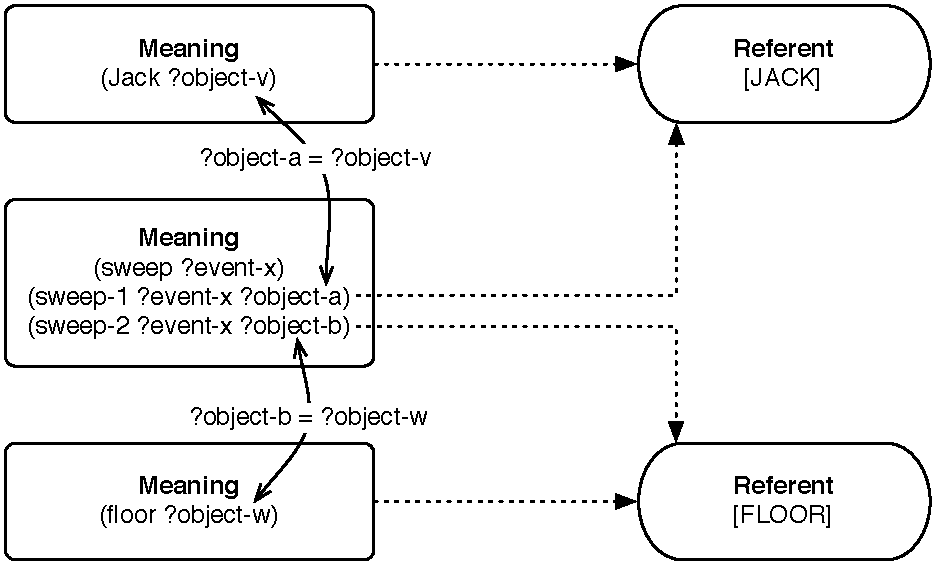
\includegraphics[width=0.8\linewidth]{Chapter2/figs/sweep-1}}
  \caption[Linking the meanings of an event]{One of the primary functions of grammar is to indicate how different meanings should be linked to each other. In the present formalization, this is represented through variable equal\is{variable equality}ities: the variables `?object-u' and `?object-a' should be made equal\is{variable equality} because they both refer to [JACK]; and the variables `?object-v' and `?object-b' should be made equal\is{variable equality} because they both refer to [FLOOR].}
   \label{f:linking}
\end{figure}

\ea
$\exists$ ?object-a, ?object-b, ?object-c, ?event-x: jack(?object-a) $\wedge$ floor(?object-b) $\wedge$ sweep(?event-x) $\wedge$ sweep-1(?event-x , ?object-a) $\wedge$ sweep-2(?event-x, ?object-b) $\wedge$ sweep-3(?event-x, ?object-c)
\item $\exists$ ?object-a, ?object-b, ?object-c, ?event-x: jack(?object-a) $\wedge$ dust(?object-b) $\wedge$ floor(?object-c) $\wedge$ sweep(?event-x) $\wedge$ sweep-1(?event-x, ?object-a) $\wedge$ sweep-2(?event-x, ?object-b) $\wedge$ sweep-3(?event-x, ?object-c)
\z

\section{A brief introduction to Fluid Construction Grammar}

\begin{figure}
\centerline{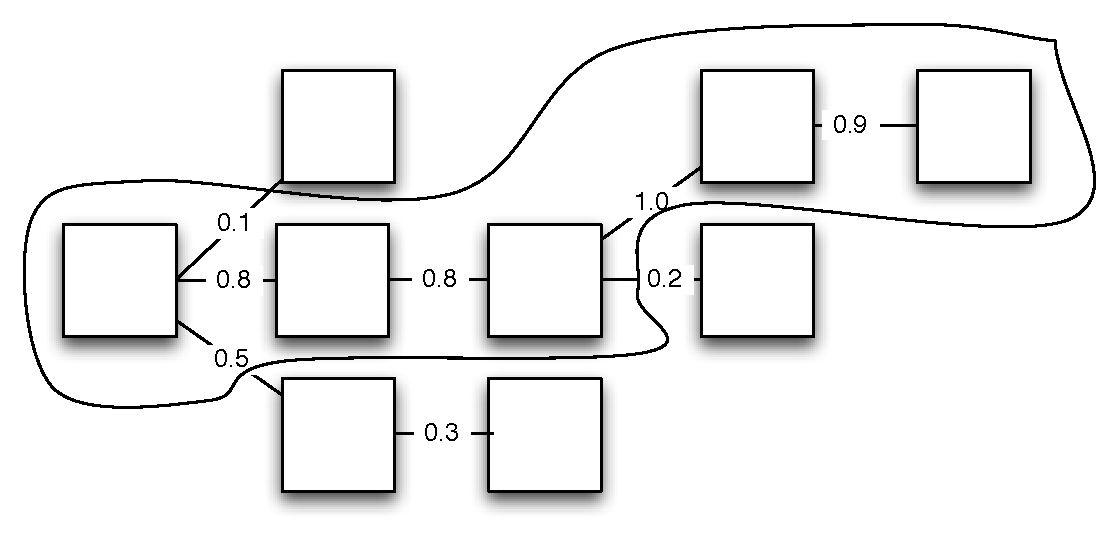
\includegraphics[width=0.8\linewidth]{Chapter2/figs/reaction-network}}
  \caption[A reaction network\is{reaction network}]{During processing, the language user builds up a reaction network\is{reaction network} by trying out constructions. The pathway with the highest confidence\is{confidence} scores is selected for producing or parsing an utterance.}
   \label{f:reaction}
\end{figure}

As already mentioned before, Fluid Construction Grammar is a computational grammar formalism for bidirectional language processing, learning and evolution. During linguistic processing, the FCG-system is either provided with a meaning that needs to be verbalized (production) or an utterance that needs to be analyzed into a meaning (parsing). The FCG-system then builds up a `reaction network\is{reaction network}' (or search tree; see Figure \ref{f:reaction}) in which each node represents a stage in the build-up of the semantic and syntactic structure of an utterance. 

Traveling from one node to the next can be achieved by applying a construction (i.e. a conventionalized mapping between meaning and form). Since there may be several hypotheses given a certain context, each link between the nodes has a `confidence\is{confidence} score' to guide the search. This score is based on (a) the (linguistic) context in which constructions can be applied, and (b) how successful the applied constructions have been in previous communicative situations. The system will in the end choose the chain with the highest estimated success.

FCG\is{construction grammar!Fluid Construction Grammar} uses many well-known techniques from computational linguistics such as term unification\is{unification} and feature structure\is{feature structure}s to represent linguistic knowledge. In fact, all linguistic knowledge (including constructions) is represented as {\bfseries coupled feature structure\is{feature structure!coupled feature structure}s}, which couple a semantic pole to a syntactic pole. All feature structure\is{feature structure}s are organized in units which are used by the basic operators of FCG\is{construction grammar!Fluid Construction Grammar} for retrieving and adding new feature-value pairs. Thus, all linguistic knowledge is represented according to the following pattern:

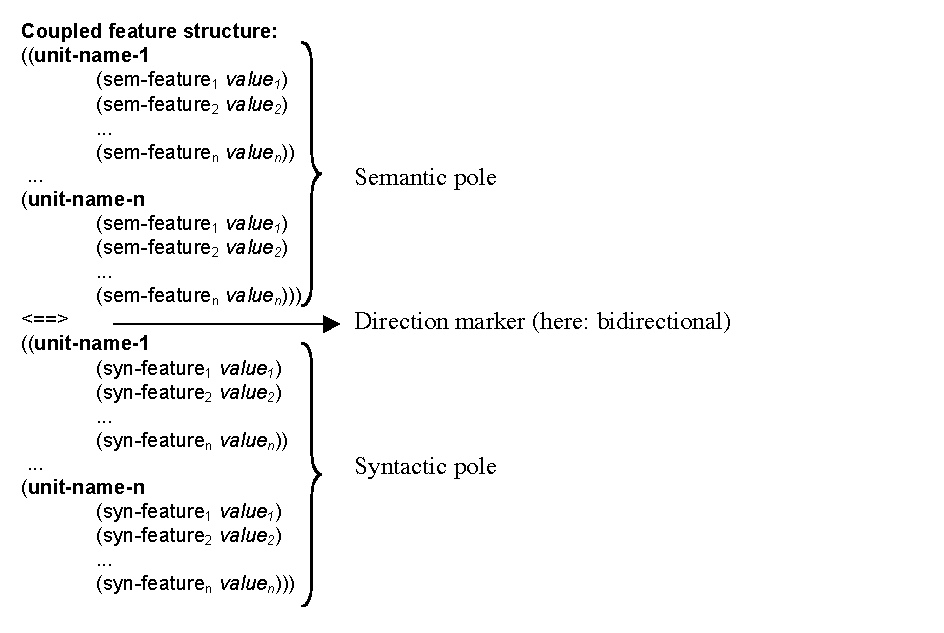
\includegraphics[width=\linewidth]{Chapter2/figs/fcg-pattern}

\begin{figure}[p]
\centerline{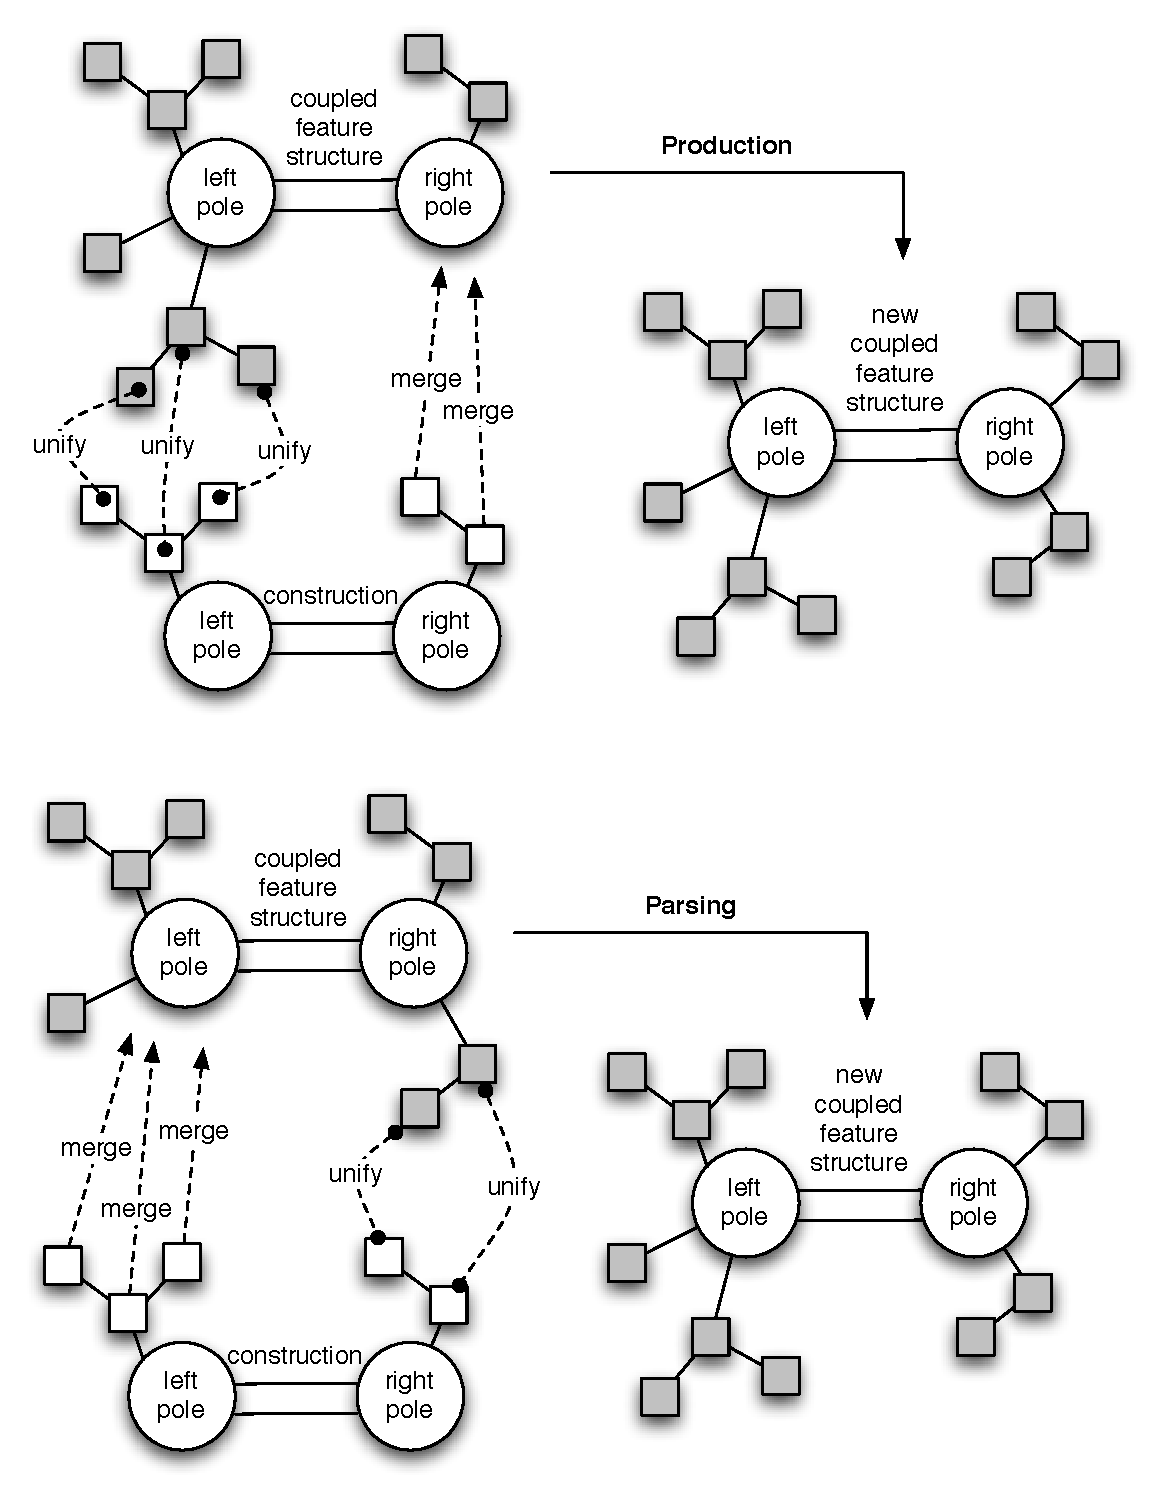
\includegraphics[width=0.8\linewidth]{Chapter2/figs/unify}}
 \caption[Unifying and merging a construction]{During production, the feature structure\is{feature structure}s (squares) in the left pole of a construction (bottom left in top figure) are unified with those of the current coupled feature structure\is{feature structure!coupled feature structure} (top left in top figure). If unification\is{unification} is successful, the right pole is merged with the coupled feature structure\is{feature structure!coupled feature structure}. This yields a new coupled feature structure\is{feature structure!coupled feature structure}, which is a new node in the reaction network\is{reaction network} (right). During parsing, the same operation is performed but this time the right pole of the construction is unified and the left one is merged with the current node.}
   \label{f:unify}
\end{figure}

\vspace{0.3cm}
\noindent{\bfseries Unify and Merge.} The two basic operations performed in FCG\is{construction grammar!Fluid Construction Grammar} are called `unify' and `merge' \citep[not to be confused with `merge' in Minimalis\is{Minimalist Program}m]{steels06unify}. These operators decide whether or not a construction can be applied in order to obtain a new node in the reaction network. `Unify' means that -- depending on the direction of processing -- the feature structure\is{feature structure} of one of the poles of a construction acts as a set of constraints that have to be compatible with the corresponding pole of the current node in the reaction network\is{reaction network}. If all the constraints are satisfied, the other pole is `merged' with the corresponding pole in the current node (unless merging fails because of conflicts in both poles). The combination of the unify\is{unify and merge} and merge operations leads to a new coupled feature structure\is{feature structure!coupled feature structure}, which is the next node in the reaction network\is{reaction network} (see Figure \ref{f:unify}).

Constructions can be applied bidirectional\is{bidirectionality}ly using the same operations, so parsing and production use the same linguistic knowledge but in opposite directions. Achieving both production and parsing is a non-trivial problem, and some formalisms therefore focus exclusively on either production or parsing (e.g. Embodied Construction Grammar). FCG\is{construction grammar!Fluid Construction Grammar} makes no claim that {\em all} linguistic knowledge is bidirectional\is{bidirectionality}, but uses bidirectional\is{bidirectionality} application of constructions for coupling input to output so that agents equipped with FCG can act both as speakers and as hearers. 

When in production mode, the FCG-system unifies the left pole of a construction (typically the semantic pole) with that of the current node; and if successful it merges the right pole (typically the syntactic pole) with that of the current node. During parsing, exactly the same linguistic items are used, but this time in the opposite direction: here, the right pole has to unify\is{unify and merge} with the corresponding pole in the current node after which the left pole can be merged with its corresponding pole in the current node.
\\
\\
\noindent{\bfseries Structure building.} FCG has a special operator -- called the `J-operator' -- for specifying hierarchical relations between units. Roughly speaking, all units marked with a J-operator\is{structure building!J-operator} are ignored during the unification\is{unification} phase, but are added or merged during the merge operation. I will limit my discussion here to the functions of the J-operator\is{structure building!J-operator} that are relevant for the constructions in this chapter. For a more technical specification, see \citet[chapter 4]{debeule07compositionality} and \citet{debeule05hierarchy}. The basic syntax of the J-operator is shown in example \ref{ex:j-operator}.

\ea
\label{ex:j-operator}
\footnotesize{\begin{verbatim}
((J ?unit ?parent (?child-1 ... ?child-n))
  (feature-1 value-1)
  ...
  (feature-n value-n))
\end{verbatim}}
\z

In this syntax, the variable `?unit' has to be bound to some unit in the coupled feature structure\is{feature structure!coupled feature structure}. If the unification\is{unification} phase did not yield a binding for this variable yet, a new unit will be built. This unit is then made a sub-unit of the unit that matches with the second argument of the J-operator\is{structure building!J-operator}. In this example this is the unit that is bound to the variable `?parent'. The J-operator\is{structure building!J-operator} can also take an optional third argument, which is a list of the units which have to be made sub-units of the unit that is bound to the first argument of the J-operator\is{structure building!J-operator} (?unit). Next, additional feature-value pairs can be listed which are merged to the structure by the J-operator\is{structure building!J-operator}. I will illustrate the J-operator\is{structure building!J-operator} through an example. Suppose that we only have the top-unit on one of the poles in the coupled feature structure\is{feature structure!coupled feature structure} and that there is a construction containing the following J-unit:

{\footnotesize\begin{verbatim}
((J ?new-unit ?top-unit))
\end{verbatim}
}

Since there is no unit yet which could have been bound to the variable ?new-unit during the unification\is{unification} phase, a new unit is created. This unit is then made a sub-unit of the unit that is bound to the second argument of the J-operator\is{structure building!J-operator} so that we get the following structure:

\ea
\Tree[.Top-unit New-unit ]
\z

Suppose now that another construction applies which contains the following J-unit:

{\footnotesize\begin{verbatim}
((J ?another-new-unit ?top-unit (?new-unit)))
\end{verbatim}}

Let's assume that the variable ?top-unit was bound by the unifier to `top-unit' and that the variable `?new-unit' was already bound to `new-unit' (which depends on the unification\is{unification} of the units that were not marked by the J-operator\is{structure building!J-operator}). The variable `?another-new-unit' does not have a binding yet so a new unit is built, which is made a sub-unit of `top-unit'. This time there is also a third argument of the J-operator\is{structure building!J-operator}. All the units in this list are made sub-units of the newly created unit so we get the following structure:

\ea
\Tree[.Top-unit [.Another-new-unit New-unit ] ]
\z

Another use of the J-operator\is{structure building!J-operator} that is adopted in this thesis is the possibility of merging additional feature-value pairs to an existing unit. This can be done as follows:

{\footnotesize\begin{verbatim}
((J ?unit NIL)
  (feature-1 value-1)
  ...
  (feature-n value-n))
\end{verbatim}}

If the second argument of the J-operator\is{structure building!J-operator} is an empty list (NIL), no structure building operation needs to be performed. In this case, the J-operator\is{structure building!J-operator} will only try to merge the feature-value pairs that are specified with the structure of the unit which is bound to the first argument of the J-operator\is{structure building!J-operator} (?unit). This functionality is needed because it allows the merging of new feature-value pairs on the same pole after successful unification\is{unification} rather than only merging the other pole of the construction to the coupled feature structure\is{feature structure!coupled feature structure}. In other words, it allows a construction to add both semantic {\em and} syntactic feature-value pairs to the coupled feature structure\is{feature structure!coupled feature structure}.

It should be noted that the above tree-like representation of hierarchical structure is only a visualization. The units of a construction or coupled feature structure are only elements of a flat list and are themselves not hierarchically organized. Instead, hierarchical relations in the linguistic structure are explicitly represented as feature-value pairs using the feature `sem-subunits' on the semantic pole and the feature `syn-subunits' on the syntactic pole.

\section{Parsing ``Jack sweep dust off-floor''}

With the meaning representation and FCG\is{construction grammar!Fluid Construction Grammar} overview in mind, we can now dive into more details of the operationalization. This section illustrates parsing using the sentence {\em Jack sweep dust off- floor} is parsed, which is a simplification of the sentence {\em Jack sweeps the dust off the floor}. Obviously, this section does not provide a description of an actual English utterance, but only highlights the problem of argument realization while ignoring issues such as agreement, determination, and so on.

At the beginning of the parsing process, the FCG-system creates a first node in a reaction network\is{reaction network}, which is a coupled feature structure\is{feature structure!coupled feature structure} with an empty semantic and syntactic pole. I assume here that the utterance is segmented into the separate strings ``jack'', ``sweep'', ``dust'', ``off-'' and ``floor''. These strings are all lumped together along with the observed word order\is{word order} (i.e. the `meets'-constraints) into the form-feature of one unit on the syntactic pole, which I will call the top-unit. The label `top-unit' is arbitrary but makes interpretation easier for human readers. On  the semantic pole, the corresponding unit (also called `top-unit') is still empty:
\\
\\
{\footnotesize{\tt <Node-1: coupled-feature-structure
\\ ((top-unit))
\\ <==>
\\ ((top-unit
\\ \hspace*{5mm} (form 
\\ \hspace*{12mm}((string jack-unit ``jack'') (string sweep-unit ``sweep'')
\\ \hspace*{13mm} (string dust-unit ``dust'') (string off-unit ``off-'')
\\ \hspace*{13mm} (string floor-unit ``floor'') (meets jack-unit sweep-unit)
\\ \hspace*{13mm} (meets sweep-unit dust-unit) (meets dust-unit off-unit)
\\ \hspace*{13mm} (meets off-unit floor-unit)))))>}}

\subsection{Unifying and merging lexical entries}
\label{s:example-parsing}

In the next step, the FCG-system performs a lexical look-up for all the words in the utterance. For this, we need a lexical entries (also called lexical constructions). The lexical entr\is{lexical entry}y for {\em jack} looks as follows: 
\\
\\
{\footnotesize{\tt <Lexical entry: jack
\\ ((?top-unit
\\ \hspace*{5mm} (meaning (== (jack ?object-1))))
\\ \hspace*{2mm}((J ?new-unit ?top-unit)
\\ \hspace*{5mm} (referent ?object-1)
\\ \hspace*{5mm} (sem-cat animate\is{animacy}-object)))
\\ <==>
\\ ((?top-unit
\\ \hspace*{5mm} (form (== (string ?new-unit ``jack''))))
\\ \hspace*{2mm}((J ?new-unit ?top-unit)
\\ \hspace*{5mm} (syn-cat (== (pos noun\is{noun})))))>}}
\\
\\
Note that the lexical entr\is{lexical entry}y for {\em jack} contains variable\is{logic variable}s not only for the meaning but also for the unit-names. The unification\is{unification} engine of FCG\is{construction grammar!Fluid Construction Grammar} can use these variable\is{logic variable}s to match them against the unit-structure of the current node in the reaction network\is{reaction network}. Since we're in parsing mode, the right pole of the entry (under the directional marker {\tt <==>}) needs to be unified with the right-pole of node-1. The right pole specifies that there has to be some unit ({\tt ?top-unit}) which must contain the feature {\tt form}, which itself must contain in its value the feature-value {\tt (string ?new-unit ``jack'')}. These constraints are indeed satisfied: the variable {\tt ?top-unit} can be bound to the unit {\tt top-unit} in the current node because it fulfills all the necessary conditions.

Since unification\is{unification} is successful, the left pole, which contains the meaning of the lexical entr\is{lexical entry}y, can be merged with the left pole of node-1. The units that are marked with the J-operator\is{structure building!J-operator} were ignored during the unification\is{unification} phase, but are now integrated: the J-operator\is{structure building!J-operator} pulls the lexical information for {\em jack} down into a new unit and specifies that this new-unit is a sub-unit of the top-unit. The J-operator\is{structure building!J-operator} also merges additional features with this new unit concerning its referent and its semantic and syntactic categorization. One could devise many other categorizations and features for {\em jack}, but they are not necessary for understanding the example here so they are left out for convenience's sake.

Since both unification\is{unification} and merge were successful, a new node is created in the reaction network\is{reaction network}. Here we see that the other words are still in the top-unit, but that there is a new unit for {\em jack} (which I conveniently label `jack-unit' here but this may be any arbitrary symbol) both in the semantic and in the syntactic pole:
\\
\\
{\footnotesize{\tt <Node-2: coupled-feature-structure
\\ ((top-unit
\\ \hspace*{5mm} (sem-subunits (jack-unit)))
\\ \hspace*{2mm}(jack-unit
\\ \hspace*{5mm} (meaning ((jack ?object-1)))
\\ \hspace*{5mm} (referent ?object-1)
\\ \hspace*{5mm} (sem-cat animate\is{animacy}-object)))
\\ <==>
\\ ((top-unit
\\ \hspace*{5mm} (syn-subunits (jack-unit))
\\ \hspace*{5mm} (form 
\\ \hspace*{10mm} ((string sweep-unit ``sweep'') (string dust-unit ``dust'') 
\\ \hspace*{11mm} (string off-unit ``off-'') (string floor-unit ``floor'') 
\\ \hspace*{11mm} (meets jack-unit sweep-unit) (meets sweep-unit dust-unit) 
\\ \hspace*{11mm} (meets dust-unit off-unit) (meets off-unit floor-unit))))
\\ \hspace*{2mm}(jack-unit
\\ \hspace*{5mm} (form ((string jack-unit ``jack'')))
\\ \hspace*{5mm} (syn-cat ((pos noun\is{noun})))))>}}
\\
\\
The lexical entr\is{lexical entry}ies for {\em dust} and {\em floor} look almost exactly the same, apart from their semantic categorization and meaning. Both entries also unify\is{unify and merge} and merge successfully with the current node and build new nodes in the reaction network\is{reaction network}: 
\\
\\
{\footnotesize{\tt <Lexical entry: dust
\\ ((?top-unit
\\ \hspace*{5mm} (meaning (== (dust ?object-2))))
\\ \hspace*{2mm}((J ?new-unit ?top-unit)
\\ \hspace*{5mm} (referent ?object-2)
\\ \hspace*{5mm} (sem-cat moveable-object)))
\\ <==>
\\ ((?top-unit
\\ \hspace*{5mm} (form (== (string ?new-unit ``dust''))))
\\ \hspace*{2mm}((J ?new-unit ?top-unit)
\\ \hspace*{5mm} (syn-cat (== (pos noun\is{noun})))))>}
\\
\vspace*{2mm}
\\
{\tt <Lexical entry: floor
\\ ((?top-unit
\\ \hspace*{5mm} (meaning (== (dust ?object-3))))
\\ \hspace*{2mm}((J ?new-unit ?top-unit)
\\ \hspace*{5mm} (referent ?object-3)
\\ \hspace*{5mm} (sem-cat surface-object)))
\\ <==>
\\ ((?top-unit
\\ \hspace*{5mm} (form (== (string ?new-unit ``floor''))))
\\ \hspace*{2mm}((J ?new-unit ?top-unit)
\\ \hspace*{5mm} (syn-cat (== (pos noun\is{noun})))))>}}\\
\\
The lexical entr\is{lexical entry}y for {\em sweep}, however, is a bit more complicated. Its main function is the same as for the other lexical entr\is{lexical entry}ies: given the string ``sweep'', it will merge the meaning of this word with the semantic pole of the current node in the reaction network\is{reaction network}. The main difference with the other words lies in the semantic and syntactic categorization of {\em sweep}. Take a look at the features `syn-frame' in the syntactic pole and `sem-frame' in the semantic pole:
\\
\\
{\tt <Lexical entry: sweep
\\ ((?top-unit
\\ \hspace*{5mm} (meaning (== (sweep ?event-x)
\\ \hspace*{32mm}(sweep-1 ?event-x ?obj-x)
\\ \hspace*{32mm}(sweep-2 ?event-x ?obj-y)
\\ \hspace*{32mm}(sweep-2 ?event-x ?obj-z))))
\\ \hspace*{2mm}((J ?new-unit ?top-unit)
\\ \hspace*{5mm} (sem-frame (== (sem-role-agent ?unit-a ?obj-x)
\\ \hspace*{36mm}(sem-role-surface ?unit-b ?obj-y)
\\ \hspace*{36mm}(sem-role-moveable ?unit-c ?obj-y)
\\ \hspace*{36mm}(sem-role-source ?unit-d ?obj-z)))))
\\ <==>
\\ ((?top-unit
\\ \hspace*{5mm} (form (== (string ?new-unit ``sweep''))))
\\ \hspace*{2mm}((J ?new-unit ?top-unit)
\\ \hspace*{5mm} (syn-cat (== (pos verb\is{verb})))
\\ \hspace*{5mm} (syn-frame (== (syn-role-subject ?unit-1)
\\ \hspace*{36mm}(syn-role-object ?unit-2)
\\ \hspace*{36mm}(syn-role-oblique ?unit-3)))))>}
\\
\\
At first glance, it seems that the lexical entr\is{lexical entry}y contains a predicate or case frame that lists the valence of a verb\is{verb} as in traditional lexicalis\is{lexicalist}t approaches. The big difference with most other approaches is however that these frames do not directly list the \is{event structure}argument structure of the verb\is{verb} but only its {\bfseries potential valent\is{valency!potential valents}s}. For example, the syn-frame only states that {\em sweep} can occur in an \is{event structure}argument structure in which there may be some unit playing the role of subject\is{syntactic role!subject}, some unit playing the role of object\is{syntactic role!object}, some unit playing the role of oblique\is{syntactic role!oblique}, or several units playing a combination of these roles. None of these roles are however obligatory: the verb\is{verb} remains agnostic as to which of these valents actually should be realized or what the possible combinations may be. I will show later that it is the construction that will select from the potential valent\is{valency!potential valents}s what the {\bfseries actual valen\is{valency!actual valency}cy} of the verb\is{verb} is or will be in the utterance (also see Figure \ref{f:sweep-quadrant}).
\begin{figure}[t]
\centerline{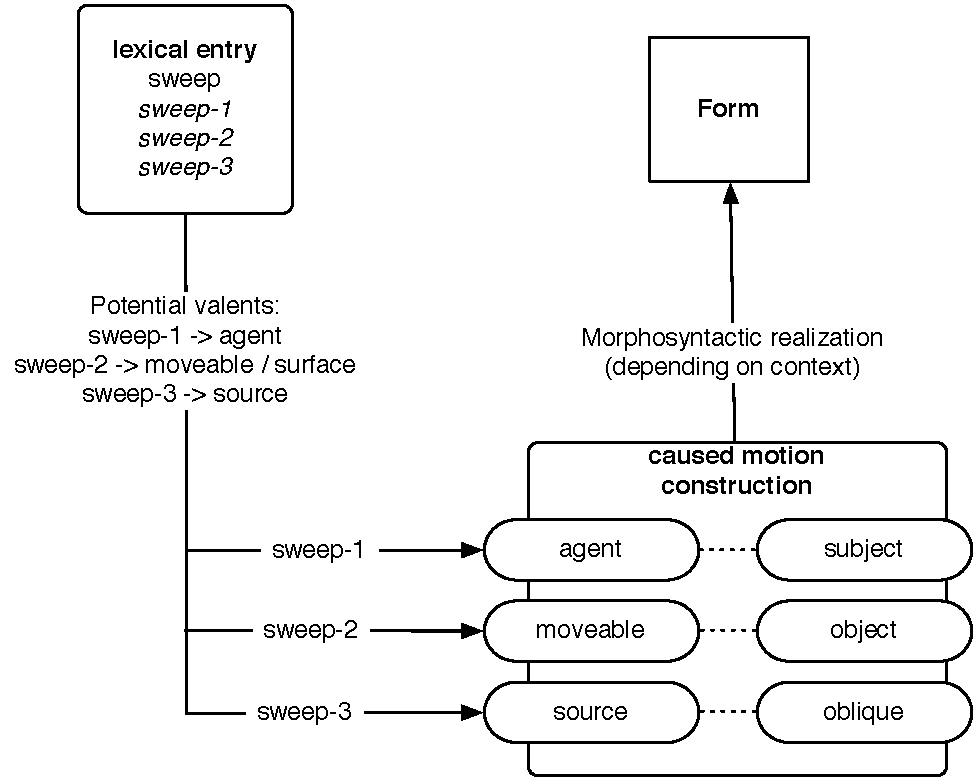
\includegraphics[width=0.8\linewidth]{Chapter2/figs/quadrant}}
 \caption[Integrating {\em sweep} with the Caused-Motion Construction]{The relation between the meaning of an event and its morphosyntactic realization is indirect and multilayered. This figure shows how a lexical entr\is{lexical entry}y introduces its `potential valent\is{valency!potential valents}s' from which the construction selects the actual valen\is{valency!actual valency}cy combination. The construction then maps this meaning onto a syntactic pattern, which in itself is realized as a certain form (depending on linguistic and extra-linguistic context)}
   \label{f:sweep-quadrant}
\end{figure}

This architecture of potential valent\is{valency!potential valents}s is mirrored in the semantic frame\is{frame!semantic frame}. Here too, the verb\is{verb} only lists all its potential valent\is{valency!potential valents}s: there may be an agent\is{semantic role!agent} role, a surface role, a moveable role, or a source\is{semantic role!source} role. The sem-frame does not specify which of these roles actually have to be realized, nor what the possible combinations are. It does specify, however, how these potential valences should be linked to the verb\is{verb}-specific participant role\is{participant role}s in the meaning feature. For example, `sem-role-agent' is linked to `sweep-1' because they share the variable `?obj-x'. `Sem-role-source' is linked to `sweep-3' because they share the variable `?obj-z'. The participant role\is{participant role} `sweep-2' is even linked to two different potential valent\is{valency!potential valents}s: `sem-role-surface' and `sem-role-moveable'. The lexical entr\is{lexical entry}y thus allows participant role\is{participant role}s to be mapped onto different semantic role\is{semantic role}s.

Both the sem- and syn-frame also contain variables that have to be bound to the unit-names of the arguments to which the roles may be assigned later on. For example, the variable `?unit-1' should be bound to the unit that plays the role of subject\is{syntactic role!subject} (if present). Notice, however, that this variable is not the same one as the variable name of the unit that may play the agent\is{semantic role!agent} role (if present): `?unit-a'. In most other grammar formalisms, such as HPSG\is{Head-Driven Phrase Structure Grammar}, a direct link between `agent\is{semantic role!agent}' and `subject\is{syntactic role!subject}' is assumed and alternating \is{event structure}argument structures such as passive\is{construction!passive construction}s are {\em deriv\is{derivation}ed} through lexical rule\is{lexical rule}s. {\bfseries I do not assume such a link between subject\is{syntactic role!subject} and agent\is{semantic role!agent}}: having two different variable names reflects the fact that both can be bound to different units as is the case in the passive\is{construction!passive construction} voice. I therefore consider the passive\is{construction!passive construction} as an alternative \is{event structure}\is{construction!argument structure construction}argument structure construction instead of a deriv\is{derivation}ational one. An active\is{construction!active construction} construction links agent\is{semantic role!agent} and subject\is{syntactic role!subject} to each other by making their variables equal\is{variable equality}, whereas the passive\is{construction!passive construction} construction features a different pattern by making other variables equal\is{variable equality} (e.g. those of the subject\is{syntactic role!subject} and the surface role as in {\em The floor was swept}). Here again, it is the construction that decides and not the verb\is{verb}. I will return to this matter in Chapter \ref{c:impact-linguistics}.

The next two Chapters will demonstrate how these potential valents can be gradually acquired and constructed through language use. They should therefore not be seen as a rigid set of possibilities or as some set of innate categories. Instead the potential uses of a verb\is{verb} can be exten\is{extension}ded (and shrunk) if needed for communicative purposes, and each possibility may become convention\is{convention}alized or become obsolete in the speech community\is{speech population}.

Unifying and merging the lexical entr\is{lexical entry}ies for {\em sweep}, {\em floor} and {\em dust} (the ordering does not matter) will lead the hearer to a fifth node in the reaction network\is{reaction network}:
\\
\\
{\footnotesize{\tt <Node-5: coupled-feature-structure
\\ ((top-unit
\\ \hspace*{5mm} (sem-subunits (jack-unit sweep-unit dust-unit floor-unit)))
\\ \hspace*{2mm}(jack-unit
\\ \hspace*{5mm} (meaning ((jack ?object-1)))
\\ \hspace*{5mm} (referent ?object-1)
\\ \hspace*{5mm} (sem-cat animate\is{animacy}-object))
\\ \hspace*{2mm}(sweep-unit
\\ \hspace*{5mm} (meaning ((sweep ?event-x)
\\ \hspace*{27mm}(sweep-1 ?event-x ?obj-x)
\\ \hspace*{27mm}(sweep-2 ?event-x ?obj-y)
\\ \hspace*{27mm}(sweep-3 ?event-x ?obj-z)))
\\ \hspace*{5mm} (sem-frame ((sem-role-agent ?unit-a ?obj-x)
\\ \hspace*{30mm}(sem-role-surface ?unit-b ?obj-y)
\\ \hspace*{30mm}(sem-role-moveable ?unit-c ?obj-y)
\\ \hspace*{30mm}(sem-role-source ?unit-d ?obj-z))))
\\ \hspace*{2mm}(dust-unit
\\ \hspace*{5mm} (meaning ((dust ?object-2)))
\\ \hspace*{5mm} (referent ?object-2)
\\ \hspace*{5mm} (sem-cat moveable-object))
\\ \hspace*{2mm}(floor-unit
\\ \hspace*{5mm} (meaning ((floor ?object-3)))
\\ \hspace*{5mm} (referent ?object-3)
\\ \hspace*{5mm} (sem-cat surface-object)))
\\ <==>
\\ ((top-unit
\\ \hspace*{5mm} (syn-subunits (jack-unit sweep-unit dust-unit floor-unit))
\\ \hspace*{5mm} (form 
\\ \hspace*{10mm}((string off-unit ``off-'') (meets jack-unit sweep-unit)
\\ \hspace*{11mm} (meets sweep-unit dust-unit) (meets dust-unit off-unit)  
\\ \hspace*{11mm} (meets off-unit floor-unit))))
\\ \hspace*{2mm}(jack-unit
\\ \hspace*{5mm} (form ((string jack-unit ``jack'')))
\\ \hspace*{5mm} (syn-cat ((pos noun\is{noun}))))
\\ \hspace*{2mm}(sweep-unit
\\ \hspace*{5mm} (form ((string sweep-unit ``sweep'')))
\\ \hspace*{5mm} (syn-cat ((pos verb\is{verb})))
\\ \hspace*{5mm} (syn-frame ((syn-role-subject ?unit-1)
\\ \hspace*{30mm}(syn-role-object ?unit-2)
\\ \hspace*{30mm}(syn-role-oblique ?unit-3))))
\\ \hspace*{2mm}(dust-unit
\\ \hspace*{5mm} (form ((string dust-unit ``dust'')))
\\ \hspace*{5mm} (syn-cat ((pos noun\is{noun}))))
\\ \hspace*{2mm}(floor-unit
\\ \hspace*{5mm} (form ((string floor-unit ``floor'')))
\\ \hspace*{5mm} (syn-cat ((pos noun\is{noun})))))>}}
\\
\\
The meanings in the above coupled feature structure\is{feature structure!coupled feature structure} are however still unlinked (see section \ref{s:linking}). In other words, the hearer knows at this stage the meaning of the individual words, but not who is doing what in the sweep-event: the variables that accompany the meaning of {\em sweep} (`?obj-x', `?obj-y' and `?obj-z') are not shared by any of the arguments (`?object-1', `?object-2' and `?object-3'). We therefore need to unify\is{unify and merge} and merge the correct construction that is able to handle the unresolved variable equalities.

\subsection{A syntactic case marker\is{case!case marking}}
\label{s:morph-rule}

Before that construction is applied, there is still the string ``off-'' in the top-unit that needs to be parsed. In this example I analyze {\em off-} as some kind of simple case marker\is{case!case marking} that assigns the oblique\is{syntactic role!oblique} case to the argument that immediately follows it. By treating {\em off-} as a case marker\is{case!case marking} I can immediately illustrate how marker\is{case!case marking}s are represented in the experiments as well.

In line with its definition in section \ref{s:stage4}, a syntactic case marker\is{case!case marking} is dissociat\is{dissociation}ed from a particular semantic role\is{semantic role}. I therefore implement case marker\is{case!case marking}s in a morphological rule or construction (a `morph-rule') in which both the left and the right pole are syntactic (so both poles operate on the syntactic pole of the current node in the reaction network\is{reaction network}). One could say in this approach that a case marker\is{case!case marking} has a syntactic or grammatical meaning rather than a semantic one. The notion of potential valent\is{valency!potential valents}s can also be applied to capture the polysemous nature of case marker\is{case!case marking}s, but for simplicity's sake I will assume here that there is a one-to-one mapping between the syntactic role\is{syntactic role} `oblique' and the marker\is{case!case marking} {\em off-}.

The morph-rule specifies that, during parsing, there needs to be a unit which contains in its form-feature the string ``off-'' and a word order\is{word order} constraint that says that the marker\is{case!case marking} immediately precedes (`meets') some other unit. If this unifies (and it does with the right pole of node-5), the left pole merges with the syntactic pole of the current node in the reaction network\is{reaction network}. The information added here is that the role of oblique\is{syntactic role!oblique} is assigned to the other unit (which immediately followed the marker\is{case!case marking}). Note that this other unit should already be present in the current node as a sub-unit of the top-unit. This is indeed the case: the variable `?some-unit' can be bound to `floor-unit' which was already present after unify\is{unify and merge}ing and merging the lexical entr\is{lexical entry}y of {\em floor}.

The morph-rule also contains a two-legged operation using the J-operator\is{structure building!J-operator}: in a first step, a new unit is created for {\em off-}, and in a second step the J-operator\is{structure building!J-operator} specifies that the newly-made unit must become a sub-unit of the other unit that immediately followed it (floor-unit). Without repeating the entire coupled feature structure\is{feature structure!coupled feature structure}, the syntactic structure now looks as follows:
\\
\\
\centerline{\Tree [ .top-unit jack-unit sweep-unit dust-unit [ .floor-unit off-unit ] ]}
\\
\\
The morphological rule itself looks as follows:
\\
\\
{\footnotesize{\tt <Morph-rule: off-
\\ ((?top-unit
\\ \hspace*{5mm} (syn-subunits (== ?some-unit)))
\\ \hspace*{2mm}(?some-unit
\\ \hspace*{5mm} (syn-role syn-role-oblique)))
\\ <==>
\\ ((?top-unit
\\ \hspace*{5mm} (form (== (string ?marker-unit ``off-'')
\\ \hspace*{24mm} (meets ?marker-unit ?some-unit))))
\\ \hspace*{2mm}((J ?marker-unit ?top-unit))
\\ \hspace*{2mm}((J ?some-unit ?top-unit (?marker-unit))))>}}


\subsection{The cause\is{causality}d motion construction\is{construction!caused motion construction}}

The utterance {\em Jack sweeps the dust off the floor} is a typical example of the cause\is{causality}d motion construction\is{construction!caused motion construction} \citep[chapter 7]{goldberg95construction}, which here carries the meaning of `X cause\is{causality}s Y to move Z by sweeping'. In the semantic pole, the construction selects from the verb\is{verb} the semantic role\is{semantic role}s of agent\is{semantic role!agent}, moveable patient\is{semantic role!patient} and source\is{semantic role!source}. On the syntactic pole it assigns the syntactic role\is{syntactic role}s of subject\is{syntactic role!subject}, object\is{syntactic role!object} and oblique\is{syntactic role!oblique} to the arguments. The construction looks as follows:
\\
\\
{\footnotesize{\tt <Construction: caused-motion
\\ ((?top-unit
\\ \hspace*{5mm} (sem-subunits (== ?unit-a ?unit-b ?unit-c ?unit-d)))
\\ \hspace*{2mm}(?unit-a
\\ \hspace*{5mm} (sem-frame (== (sem-role-agent ?unit-b ?obj-x)
\\ \hspace*{36mm}(sem-role-moveable ?unit-c ?obj-y)
\\ \hspace*{36mm}(sem-role-source ?unit-d ?obj-z))))
\\ \hspace*{2mm}(?unit-b
\\ \hspace*{5mm} (referent ?obj-x)
\\ \hspace*{5mm} (sem-cat animate\is{animacy}-object))
\\ \hspace*{2mm}(?unit-c
\\ \hspace*{5mm} (referent ?obj-y)
\\ \hspace*{5mm} (sem-cat moveable-object))
\\ \hspace*{2mm}(?unit-d
\\ \hspace*{5mm} (referent ?obj-z)))
\\ <==>
\\ ((?top-unit
\\ \hspace*{5mm} (syn-subunits (== ?unit-a ?unit-b ?unit-c ?unit-d))
\\ \hspace*{5mm} (form ((meets ?unit-b ?unit-a) (meets ?unit-a ?unit-c)
\\ \hspace*{19mm} (meets ?unit-c ?unit-d))))
\\ \hspace*{2mm}(?unit-a
\\ \hspace*{5mm} (syn-cat (== (pos verb\is{verb})))
\\ \hspace*{5mm} (syn-frame (== (syn-role-subject ?unit-b)
\\ \hspace*{36mm}(syn-role-object ?unit-c)
\\ \hspace*{36mm}(syn-role-oblique ?unit-d))))
\\ \hspace*{2mm}(?unit-d
\\ \hspace*{5mm} (syn-role syn-role-oblique))
\\ \hspace*{2mm}((J ?unit-b NIL)
\\ \hspace*{5mm} (syn-role syn-role-subject))
\\ \hspace*{2mm}((J ?unit-c NIL) 
\\ \hspace*{5mm} (syn-role syn-role-object)))>}}
\\
\\
Since the hearer is parsing, the right pole needs to be unified with the current node in the reaction network\is{reaction network}. The right pole here demands there to be some unit with at least four sub-units and with a certain word order\is{word order} among them (i.e. the `meets'-constraints). The last argument also has to have the syntactic role\is{syntactic role} of oblique\is{syntactic role!oblique}. The right pole of the current node satisfies all the constraints: jack-unit receives subject\is{syntactic role!subject} status and dust-unit becomes the object. The unit for {\em floor} was already marked as oblique\is{syntactic role!oblique} by the morphological rule that was shown in the previous section.

Thanks to the word-order constraints, the construction can unambiguously bind the variables `?unit-b' to `jack-unit', `?unit-c' to `dust-unit' and `?unit-d' to `floor-unit'. The construction then links the syntactic role\is{syntactic role}s to the semantic role\is{semantic role}s by making the necessary variables equal\is{variable equality}: the subject\is{syntactic role!subject} jack-unit is assigned the role of agent\is{semantic role!agent}, the object\is{syntactic role!object} dust-unit is assigned the role of moveable (object) and the oblique\is{syntactic role!oblique} floor-unit is assigned the role of source\is{semantic role!source}. By doing so, the construction can also link the meanings to each other: sem-role-agent shares the variable `?obj-x' with sweep-1 and the referent of jack-unit, sem-role-moveable shares the variable `?obj-y' with sweep-2 and the referent of dust-unit, and sem-role-source shares the variable `?obj-z' with sweep-3 and the referent of floor-unit. This leads to the following node in the reaction network\is{reaction network}:
\\
\\
{\footnotesize{\tt <Node-7: coupled-feature-structure
\\ ((top-unit
\\ \hspace*{5mm} (sem-subunits (jack-unit sweep-unit dust-unit floor-unit)))
\\ \hspace*{2mm}(jack-unit
\\ \hspace*{5mm} (meaning ((jack ?obj-x)))
\\ \hspace*{5mm} (referent ?obj-x)
\\ \hspace*{5mm} (sem-role sem-role-agent)
\\ \hspace*{5mm} (sem-cat animate\is{animacy}-object))
\\ \hspace*{2mm}(sweep-unit
\\ \hspace*{5mm} (meaning ((sweep ?event-x)
\\ \hspace*{27mm}(sweep-1 ?event-x ?obj-x)
\\ \hspace*{27mm}(sweep-2 ?event-x ?obj-y)
\\ \hspace*{27mm}(sweep-3 ?event-x ?obj-z)))
\\ \hspace*{5mm} (sem-frame ((sem-role-agent jack-unit ?obj-x)
\\ \hspace*{30mm}(sem-role-surface dust-unit ?obj-y)
\\ \hspace*{30mm}(sem-role-moveable dust-unit ?obj-y)
\\ \hspace*{30mm}(sem-role-source floor-unit ?obj-z))))
\\ \hspace*{2mm}(dust-unit
\\ \hspace*{5mm} (meaning ((dust ?obj-y)))
\\ \hspace*{5mm} (referent ?obj-y)
\\ \hspace*{5mm} (sem-role sem-role-moveable)
\\ \hspace*{5mm} (sem-cat moveable-object))
\\ \hspace*{2mm}(floor-unit
\\ \hspace*{5mm} (meaning ((floor ?obj-z)))
\\ \hspace*{5mm} (referent ?obj-z)
\\ \hspace*{5mm} (sem-role sem-role-source)
\\ \hspace*{5mm} (sem-cat surface-object)))
\\ <==>
\\ ((top-unit
\\ \hspace*{5mm} (syn-subunits (jack-unit sweep-unit dust-unit floor-unit))
\\ \hspace*{5mm} (form ((meets jack-unit sweep-unit) 
\\ \hspace*{19mm} (meets sweep-unit dust-unit)
\\ \hspace*{19mm} (meets dust-unit off-unit)))) 
\\ \hspace*{2mm}(jack-unit
\\ \hspace*{5mm} (form ((string jack-unit ''jack'')))
\\ \hspace*{5mm} (syn-role syn-role-subject)
\\ \hspace*{5mm} (syn-cat ((pos noun\is{noun}))))
\\ \hspace*{2mm}(sweep-unit
\\ \hspace*{5mm} (form ((string sweep-unit ''sweep'')))
\\ \hspace*{5mm} (syn-cat ((pos verb\is{verb})))
\\ \hspace*{5mm} (syn-frame ((syn-role-subject jack-unit)
\\ \hspace*{30mm}(syn-role-object dust-unit)
\\ \hspace*{30mm}(syn-role-oblique foor-unit))))
\\ \hspace*{2mm}(dust-unit
\\ \hspace*{5mm} (form ((string dust-unit ''dust'')))
\\ \hspace*{5mm} (syn-role syn-role-object)
\\ \hspace*{5mm} (syn-cat ((pos noun\is{noun}))))
\\ \hspace*{2mm}(floor-unit
\\ \hspace*{5mm} (syn-subunits (off-unit))
\\ \hspace*{5mm} (form ((string floor-unit ''floor'')))
\\ \hspace*{5mm} (syn-role syn-role-oblique)
\\ \hspace*{5mm} (syn-cat ((pos noun\is{noun}))))
\\ \hspace*{2mm}(off-unit
\\ \hspace*{5mm} (form ((string off-unit ''off-'') 
\\ \hspace*{19mm} (meets off-unit floor-unit)))))>}}
\\
\\
Now we can extract the following meaning from the semantic pole of the coupled feature structure:

\ea
$\exists$ ?obj-x, ?obj-y, ?obj-z, ?event-x: jack(?obj-x) $\wedge$ dust(?obj-y) $\wedge$ floor(?obj-z) $\wedge$ sweep(?event-x) $\wedge$ sweep-1(?event-x , ?obj-x) $\wedge$ sweep-2(?event-x, ?obj-y) $\wedge$ sweep-3(?event-x, ?obj-z)
\z

As can be seen in the meaning, all variables that refer to the same referent have been made equal\is{variable equality} by the construction. The hearer thus knows that {\em jack} was the sweeper, that {\em dust} was the thing being swept, and that the {\em floor} was the source\is{semantic role!source} of the motion. In the experiments reported in this book, the agents will then match this parsed meaning against their world model.

\section{Producing ``jack sweep floor''}

This section gives an overview of how an utterance such as {\em jack sweep floor} can be produced in Fluid Construction Grammar\is{construction grammar!Fluid Construction Grammar}. In this case, the cause\is{causality}d motion construction\is{construction!caused motion construction} is not used, but a construction which maps the semantic frame\is{frame!semantic frame} `X acts on surface Y' onto the syntactic frame\is{frame!syntactic frame} `Subject-Verb\is{verb}-Object'. The speaker starts with the following meaning (in which NIL stands for `empty' or `not profiled\is{event profile}'):

\ea
((jack object-1) (floor object-2) (sweep event-1) 
\\ \hspace*{3mm}(sweep-1 event-1 object-1) (sweep-2 event-1 object-2) 
\\ \hspace*{3mm}(sweep-3 event-1 NIL))
\z

In order to verb\is{verb}alize this meaning, the speaker constructs a reaction network\is{reaction network}. The first node in the network is a coupled feature structure\is{feature structure!coupled feature structure} in which the entire meaning is placed into one unit in the semantic pole, and in which the syntactic pole is still empty:
\\
\\
{\footnotesize{\tt <Node-1: coupled-feature-structure
\\ ((top-unit
\\ \hspace*{5mm} (meaning ((jack object-1) (floor object-2)
\\ \hspace*{24mm} (sweep event-1) (sweep-1 event-1 object-1)
\\ \hspace*{24mm} (sweep-2 event-1 object-2) (sweep-3 event-1 NIL)))))
\\ <==>
\\ ((top-unit))>}}

\subsection{Unifying and merging lexical entr\is{lexical entry}ies}

Next, the speaker builds new nodes in the network by unify\is{unify and merge}ing and merging the lexical entr\is{lexical entry}ies that cover these meanings. Suppose that the speaker has the same lexical entr\is{lexical entry}ies as given in the previous section and that all three of them ({\em jack, sweep} and {\em floor)} are a successful match, then the new coupled feature structure\is{feature structure!coupled feature structure} looks as follows:
\\
\\
{\footnotesize{\tt <Node-4: coupled-feature-structure
\\ ((top-unit
\\ \hspace*{5mm} (sem-subunits (jack-unit sweep-unit floor-unit)))
\\ \hspace*{2mm}(jack-unit
\\ \hspace*{5mm} (meaning ((jack object-1)))
\\ \hspace*{5mm} (referent object-1)
\\ \hspace*{5mm} (sem-cat animate\is{animacy}-object))
\\ \hspace*{2mm}(sweep-unit
\\ \hspace*{5mm} (meaning ((sweep event-1)
\\ \hspace*{27mm}(sweep-1 event-1 object-1)
\\ \hspace*{27mm}(sweep-2 event-1 object-2)
\\ \hspace*{27mm}(sweep-3 event-1 NIL)))
\\ \hspace*{5mm} (sem-frame ((sem-role-agent ?unit-a object-1)
\\ \hspace*{30mm}(sem-role-surface ?unit-b object-2)
\\ \hspace*{30mm}(sem-role-moveable ?unit-c object-2)
\\ \hspace*{30mm}(sem-role-source ?unit-d NIL))))
\\ \hspace*{2mm}(floor-unit
\\ \hspace*{5mm} (meaning ((floor object-2)))
\\ \hspace*{5mm} (referent object-2)
\\ \hspace*{5mm} (sem-cat surface-object)))
\\ <==>
\\ ((top-unit
\\ \hspace*{5mm} (syn-subunits (jack-unit sweep-unit floor-unit)))
\\ \hspace*{2mm}(jack-unit
\\ \hspace*{5mm} (form ((string jack-unit ''jack'')))
\\ \hspace*{5mm} (syn-cat ((pos noun\is{noun}))))
\\ \hspace*{2mm}(sweep-unit
\\ \hspace*{5mm} (form ((string sweep-unit ''sweep'')))
\\ \hspace*{5mm} (syn-cat ((pos verb\is{verb})))
\\ \hspace*{5mm} (syn-frame ((syn-role-subject ?unit-1)
\\ \hspace*{30mm}(syn-role-object ?unit-2)
\\ \hspace*{30mm}(syn-role-oblique ?unit-3))))
\\ \hspace*{2mm}(floor-unit
\\ \hspace*{5mm} (form ((string floor-unit ''floor'')))
\\ \hspace*{5mm} (syn-cat ((pos noun\is{noun})))))>}}
\\
\\
Since the speaker knows which meaning he wants to express, there are no unresolved variable equal\is{variable equality}ities in the meanings in the semantic pole. However, so far no semantic or syntactic role\is{syntactic role}s have been assigned yet: the lexical entr\is{lexical entry}y of {\em sweep} has merely introduced its potential valent\is{valency!potential valents}s, but not its actual valen\is{valency!actual valency}cy. This is reflected by the fact that the arguments do not have the feature `sem-role' or `syn-role' yet and that there are still variables left for the unit-names in both the syn- and sem-frame. It is also still undecided which participant should be mapped onto subject\is{syntactic role!subject} and which onto object or oblique\is{syntactic role!oblique}.

\subsection{The agent-acts-on-surface construction}

Trying to unify\is{unify and merge} the cause\is{causality}d motion construction\is{construction!caused motion construction} leads to a failure: first of all, {\em floor} is categorized as a static surface-object and thus violates the construction's constraint that the patient\is{semantic role!patient} has to be moveable, and second, the source\is{semantic role!source} argument is missing. So a different construction needs to be unified and merged to travel to the next node in the network. The following `agent-acts-on-surface' construction would do the trick:

\newpage
\noindent{\footnotesize{\tt <Construction: agent-acts-on-surface
\\ ((?top-unit
\\ \hspace*{5mm} (sem-subunits (== ?unit-a ?unit-b ?unit-c)))
\\ \hspace*{2mm}(?unit-a
\\ \hspace*{5mm} (sem-frame (== (sem-role-agent ?unit-b ?obj-x)
\\ \hspace*{36mm}(sem-role-surface ?unit-c ?obj-y))))
\\ \hspace*{2mm}(?unit-b
\\ \hspace*{5mm} (referent ?obj-x)
\\ \hspace*{5mm} (sem-cat animate\is{animacy}-object))
\\ \hspace*{2mm}(?unit-c
\\ \hspace*{5mm} (referent ?obj-y)
\\ \hspace*{5mm} (sem-cat surface-object)))
\\ <==>
\\ ((?top-unit
\\ \hspace*{5mm} (syn-subunits (== ?unit-a ?unit-b ?unit-c ?unit-d))
\\ \hspace*{5mm} (form ((meets ?unit-b ?unit-a) (meets ?unit-a ?unit-c))))
\\ \hspace*{2mm}(?unit-a
\\ \hspace*{5mm} (syn-cat (== (pos verb\is{verb})))
\\ \hspace*{5mm} (syn-frame (== (syn-role-subject ?unit-b)
\\ \hspace*{36mm}(syn-role-object ?unit-c))))
\\ \hspace*{2mm}((J ?unit-b NIL)
\\ \hspace*{5mm} (syn-role syn-role-subject))
\\ \hspace*{2mm}((J ?unit-c NIL) 
\\ \hspace*{5mm} (syn-role syn-role-object)))>}}
\\
\\
First the speaker tries to unify\is{unify and merge} the semantic pole with that of the current node in the reaction network\is{reaction network}. This is a success because all the constraints are satisfied: the construction expects some unit with three sub-units, one of which is an animate\is{animacy}-object and one of which is a surface-object. The construction also selects the semantic role\is{semantic role}s of `agent\is{semantic role!agent}' and `surface' from the verb\is{verb}'s potential valent\is{valency!potential valents}s and assigns them to the correct arguments. Next, the right pole of the construction is merged with the right pole of the current node. Since it is specified that the agent\is{semantic role!agent} maps onto subject\is{syntactic role!subject} and the surface maps onto object\is{syntactic role!object} in this construction, the correct syntactic role\is{syntactic role}s are assigned to the arguments, including their word order\is{word order}. The new node looks as follows:
\\
\\
{\footnotesize{\tt <Node-5: coupled-feature-structure
\\ ((top-unit
\\ \hspace*{5mm} (sem-subunits (jack-unit sweep-unit floor-unit)))
\\ \hspace*{2mm}(jack-unit
\\ \hspace*{5mm} (meaning ((jack object-1)))
\\ \hspace*{5mm} (referent object-1)
\\ \hspace*{5mm} (sem-role sem-role-agent)
\\ \hspace*{5mm} (sem-cat animate\is{animacy}-object))
\\ \hspace*{2mm}(sweep-unit
\\ \hspace*{5mm} (meaning ((sweep event-1)
\\ \hspace*{27mm}(sweep-1 event-1 object-1)
\\ \hspace*{27mm}(sweep-2 event-1 object-2)
\\ \hspace*{27mm}(sweep-3 event-1 NIL)))
\\ \hspace*{5mm} (sem-frame ((sem-role-agent jack-unit object-1)
\\ \hspace*{30mm}(sem-role-surface floor-unit object-2)
\\ \hspace*{30mm}(sem-role-moveable floor-unit object-2)
\\ \hspace*{30mm}(sem-role-source ?unit-d NIL))))
\\ \hspace*{2mm}(floor-unit
\\ \hspace*{5mm} (meaning ((floor object-2)))
\\ \hspace*{5mm} (referent object-2)
\\ \hspace*{5mm} (sem-role sem-role-surface)
\\ \hspace*{5mm} (sem-cat surface-object)))
\\ <==>
\\ ((top-unit
\\ \hspace*{5mm} (syn-subunits (jack-unit sweep-unit floor-unit))
\\ \hspace*{5mm} (form ((meets jack-unit sweep-unit) 
\\ \hspace*{18,5mm} (meets sweep-unit floor-unit))))
\\ \hspace*{2mm}(jack-unit
\\ \hspace*{5mm} (form ((string jack-unit ''jack'')))
\\ \hspace*{5mm} (syn-role syn-role-subject)
\\ \hspace*{5mm} (syn-cat ((pos noun\is{noun}))))
\\ \hspace*{2mm}(sweep-unit
\\ \hspace*{5mm} (form ((string sweep-unit ''sweep'')))
\\ \hspace*{5mm} (syn-cat ((pos verb\is{verb})))
\\ \hspace*{5mm} (syn-frame ((syn-role-subject jack-unit)
\\ \hspace*{30mm}(syn-role-object floor-unit)
\\ \hspace*{30mm}(syn-role-oblique ?unit-3))))
\\ \hspace*{2mm}(floor-unit
\\ \hspace*{5mm} (form ((string floor-unit ''floor'')))
\\ \hspace*{5mm} (syn-role syn-role-object)
\\ \hspace*{5mm} (syn-cat ((pos noun\is{noun})))))>}}
\\
\\
The speaker has no other constructions or linguistic items that could unify\is{unify and merge} and merge, so he is almost done processing. In the final phase, he takes all the formal constraints specified in the syntactic pole of the last node and renders them into the utterance {\em jack sweep floor}.

\section{Networks and conventionalization}

The previous two sections showed how lexical and constructional meanings can integrate through the potential valent\is{valency!potential valents}s of the verb\is{verb} on the one hand, and the selection\is{selection} of the actual valen\is{valency!actual valency}cy by the constructions on the other. I also suggested that the list of potential valent\is{valency!potential valents}s can be exten\is{extension}ded if needed for communication. However, this solution is too powerful because it does not explain why speakers of English\is{English} prefer not to use {\em sweep} in for example the ditransitive\is{ditransitive clause} construction as in {\em *he swept him the dust}. We therefore need an additional strategy to restrict the powers of the proposed representation.

Utterances such as {\em *he swept him the dust} are perfectly intelligible but somehow speakers (usually) refrain from using words in constructions that they are not convention\is{convention}ally associated with. Convention or entrench\is{entrenchment}ment can intuitively be captured in a network as illustrated in Figure \ref{f:network-sweep}. The basic idea is the following: we never observe words in total isolation but always in language use. We can therefore keep links between constructions that reflect their past co-occur\is{co-occurrence}rences. For example, {\em sweep} has a link to the intransitive construction, the cause\is{causality}d motion construction\is{construction!caused motion construction}, etc. The link reflects convention\is{convention}alization through a confidence\is{confidence} score: the higher this score, the more confident the speaker feels integrating the lexical entr\is{lexical entry}y with the construction. The lower the score, the more `strain' there is to go ahead and fuse the lexical entr\is{lexical entry}y with the construction. Scores in the network can be changed each time the lexical entr\is{lexical entry}y and the construction co-occur\is{co-occurrence}: the score increases if they are used in successful communication, but decreases if co-occur\is{co-occurrence}rence leads to communicative failure. Each interaction also yields the possibility of adding new links. I will come back to the exact nature of this network in the following chapters.
\begin{figure}[tb]
\centerline{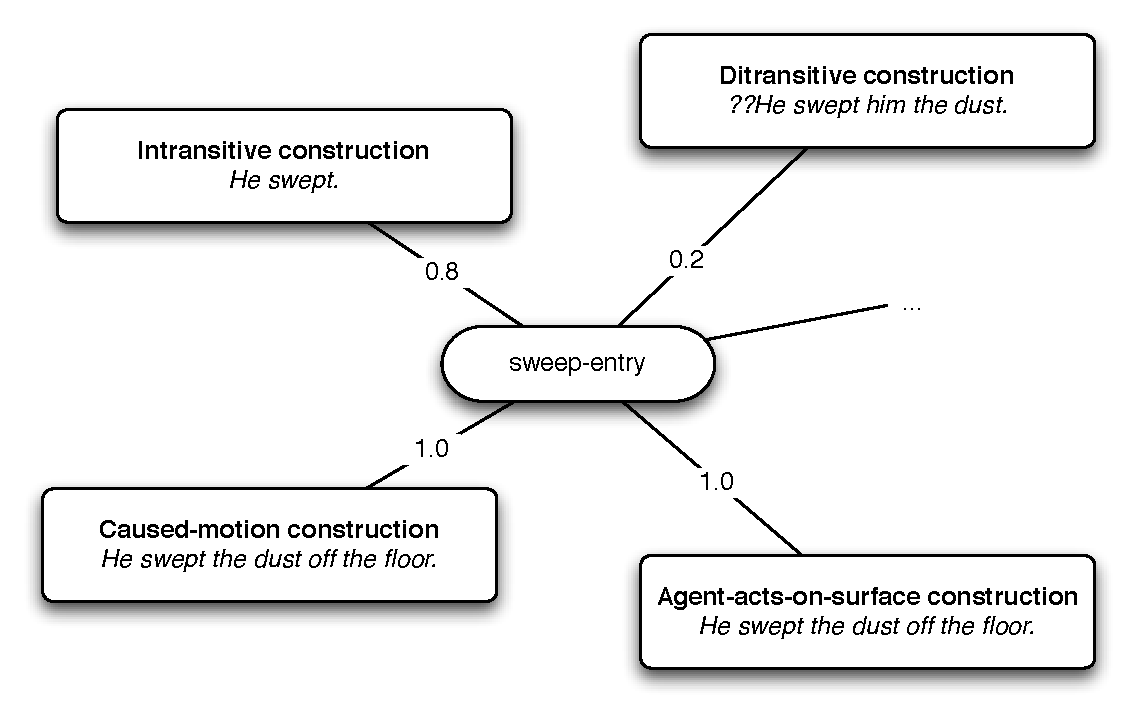
\includegraphics[width=\linewidth]{Chapter2/figs/network}}
 \caption[Network for {\em sweep}]{Lexical entries keep a link to all the constructions that they integrated with. Each link has a specific confidence\is{confidence} score which reflects how confident the language user is that the lexical entr\is{lexical entry}y can be fused with the construction. The higher the score, the more conventionalized the link is. The lower the score, the more `strain' the speaker will have to use the entry and the construction together. This network thus captures convention\is{convention}alised patterns in a language.}
   \label{f:network-sweep}
\end{figure}
